%\newpage
In this chapter, we will mainly consider two statistic models, namely
logistic regression for linearly separable sets,
and support vector machine (SVM).
These two linear models form the foundation of deep learning, since
the final fully connected output layer of a deep neural network is
often given by one of these two linear classifiers.  One main objective in this chapter is that  these linear classification models can be used to classify a collection of 
linearly separable classes.  

In the presentation of this chapter, we treat both logistic regression
and support vector machine as pure mathematical techniques for
linearly separable sets.  In the later chapters, we will relate these
techniques in the context of machine learning, especially deep
learning. 
\section{Definition of linearly separable sets}
In this section, we consider a special class of $k$ linearly separable sets for $k\ge 2$.  Let us first introduce the following
definition for binary classification. 


For $k=2$, there is a very simple geometric interpretation of two
linearly separable sets. 
\begin{definition}\label{lem:2class}
  The two sets $A_1$, $A_2\subset \mathbb{R}^d$ are linearly separable
   if there exists a hyperplane
  \begin{equation}
    \label{2classH}
H_0=\{x:wx+b=0\},    
  \end{equation}
 such that $wx+b>0$ if $x\in A_1$ and $wx+b<0$ if $x\in A_2$.
  \end{definition}
\begin{figure}
\centering
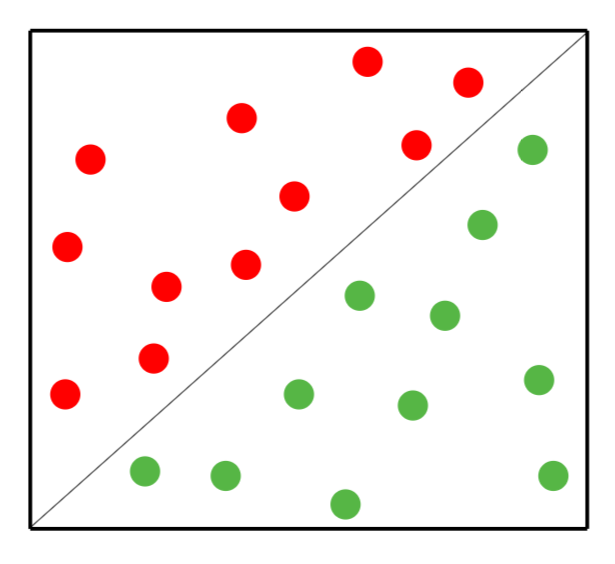
\includegraphics[width=1.5in]{LinearS1.png}  \quad  %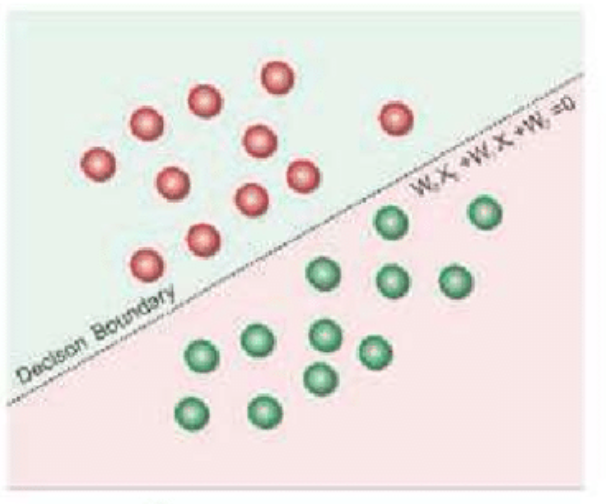
\includegraphics[width=1.5in]{LinearS2.png} 
\caption{One linearly separable set}
\label{twoclassification}
\end{figure}

\begin{figure}
\centering
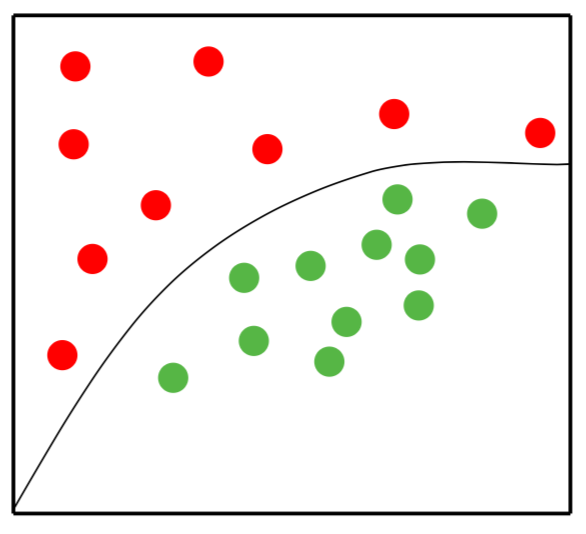
\includegraphics[width=1.5in]{NLinearS1.png}  \quad  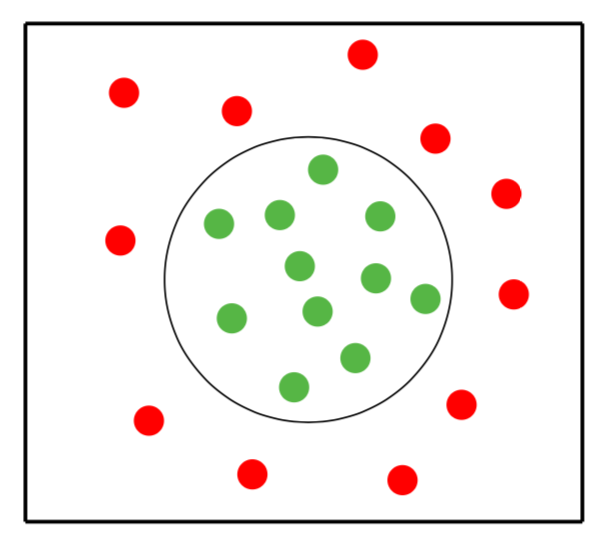
\includegraphics[width=1.5in]{NLinearS2.png} 
\caption{Two non-linearly separable sets}
\label{twoclassification}
\end{figure}

%\blankpage
%\newbreak
\begin{lemma}\label{lem:2class}
  The two sets $A_1$, $A_2\subset \mathbb{R}^d$ are linearly separable
 if there exists 
  \begin{equation}
    \label{Wb}
W=
\begin{pmatrix}
  w_1\\
w_2
\end{pmatrix}
\in \mathbb{R}^{2\times d}, 
b=
\begin{pmatrix}
  b_1\\
b_2
\end{pmatrix}
\in \mathbb{R}^{2\times d}, 
\end{equation}
such that,  % for each $1\le i\le 2$ and $ j \neq i$
\begin{equation}
\label{eq:3}
 w_1x+b_1 > w_2x+b_2,\ \forall x\in A_1,
 \end{equation}
and
\begin{equation}
\label{eq:3}
 w_1x+b_1 < w_2x+b_2,\ \forall x\in A_2.
 \end{equation}
\end{lemma}

\begin{proof}
	Here, we can just take $w = w_1 - w_2$ and $b = b_1 - b_2$, 
	then we can check that the hyperplane $wx + b$ satisfies the
	definition as presented before.
\end{proof}


%\blankpage
%\newbreak
Now let us consider multi-class classification.
To begin with the definition, let us assume that the data space is 
divided into $k$ classes represented by $k$ disjoint sets $A_1,A_2,\cdots,A_k\subset \mathbb{R}^d$, which means
\begin{equation}
A = A_1\cup A_2\cup \cdots \cup A_k, ~A_i\cap A_j = \emptyset, \forall i \neq j.
\end{equation}

\begin{definition}[Linearly Separable]
  A collection of subsets $A_1,...,A_k\subset \mathbb{R}^d$ are
  linearly separable if there exist
  \begin{equation}
    \label{Wb}
W=
\begin{pmatrix}
  w_1\\
\vdots\\
w_k
\end{pmatrix}
\in \mathbb{R}^{k\times d}, 
b=
\begin{pmatrix}
  b_1\\
\vdots\\
b_k
\end{pmatrix}
\in \mathbb{R}^{k\times d}, 
\end{equation}
such that,   for each $1\le i\le k$ and $ j \neq i$
\begin{equation}
\label{eq:3}
 w_ix+b_i > w_jx+b_j,\ \forall x\in A_i.
 \end{equation}
namely, each pairs of $A_i$ and $A_j$ are linearly separable by the plane
\begin{equation}
  \label{Hij}
H_{ij}=\{(w_i-w_j)\cdot x+(b_i-b_j) = 0\}, \quad \forall j\neq i.
\end{equation} 
\end{definition}
The geometric interpretation for linearly separable sets is less
obvious when $k>2$. 
\begin{lemma}{\label{Interplation}}
Assume that $A_1,...,A_k$ are linearly separable and $ W\in
\mathbb{R}^{k\times d} $ and $b\in\mathbb{R}^k $ satisfy \eqref{Wb}.  Define
\begin{equation}
\label{Gammai}
\Gamma_i(W,b) = \{x\in\mathbb R^d: (Wx+b)_i > (Wx+b)_j,\ \forall j \neq i\}     
\end{equation}
Then for each $i$, 
\begin{equation}
  \label{AiGamma}
A_i \subset \Gamma_i(W,b)  
\end{equation}
\end{lemma}
We note that  each $\Gamma_i(W,b)  $ is a polygon whose boundary consists of hyperplanes given by 
\eqref{Hij}.
\begin{figure}
\centering
	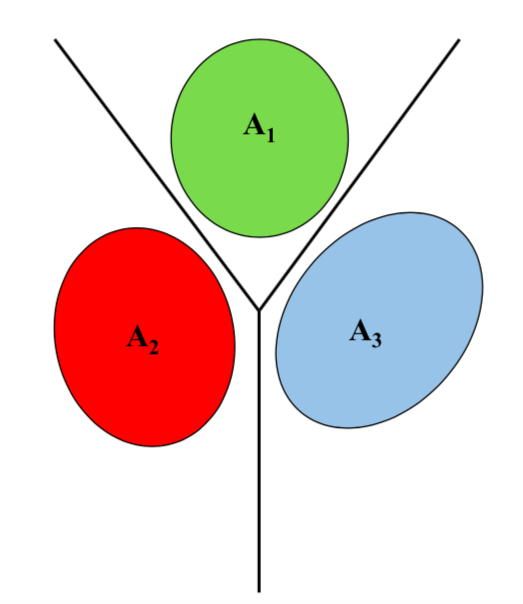
\includegraphics[width=1.5in]{./figures/3-class.PNG}
	\caption{Linearly separable sets in 2-d space (k = 3)}
	\label{twoclassification}
\end{figure}

We next introduce two more definitions of linearly separable sets that
have more clear geometric interpretation. 

\begin{definition}[All-vs-One Linearly Separable]
 A collection of subsets $A_1,...,A_k\subset \mathbb{R}^d$ is
 all-vs-one linearly separable
if for each $i = 1,...,k$, 
$A_i$ and $\displaystyle \cup_{j\neq i} A_j$ are linearly separable. 
\end{definition}

\begin{figure}[H]
\centering
	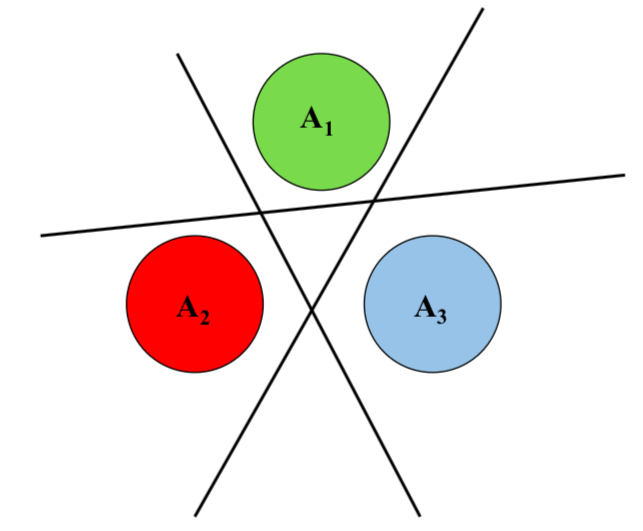
\includegraphics[width=1.5in]{./figures/MulLClassfication.PNG}
	\caption{All-vs-One linearly separable sets (k = 3)}
	\label{twoclassification}
\end{figure}

\begin{definition}[Pairwise Linearly Separable]
  A collection of subsets $A_1,...,A_k\subset \mathbb{R}^d$ is
  pairwise linearly separable if for each pair of indices $1\leq i <
  j\leq k$, 
$A_i$ and $A_j$ are linearly separable. 
\end{definition}



\begin{figure}[H]
\centering
	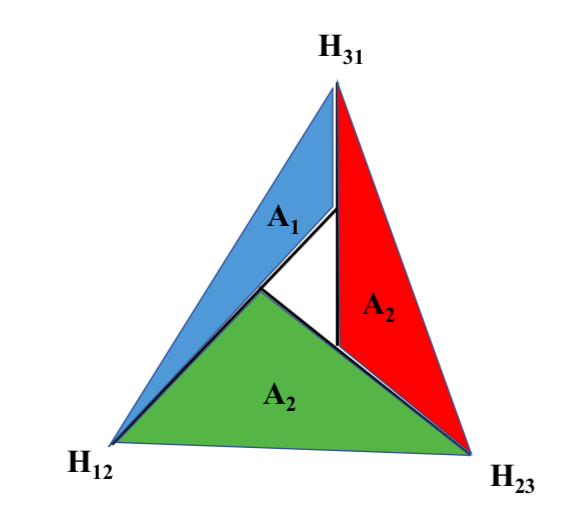
\includegraphics[width=1.5in]{./figures/pairwise_linearly_separable.png}
	\caption{Pairwise linearly separable sets in 2-d space (k = 3)}
	\label{pairwise_separable_example}
\end{figure}


We begin by comparing our notion of linearly separable to the two
other previously introduced geometric definitions of all-vs-one
linearly separable and pairwise lineaerly separable.  Obviously, in
the case of two classes, they are all equivalent, however, with more
than two classes this is no longer the case. We do have the following
implications, though.

\begin{lemma}
  If $A_1,...,A_k\subset \mathbb{R}^d$ are all-vs-one linearly
  separable, then they are linearly separable as well.
\end{lemma}
\begin{proof}
 Assume that $A_1,...,A_k$ are all-vs-one linearly separable. For each $i$, let $w_i$, $b_i$ be such that $w_ix + b_i$ separates
 $A_i$ from $\cup_{j\neq i} A_j$, i.e. $w_ix + b_i > 0$ for $x\in A_i$ and $w_ix + b_i < 0$ for $x \in \cup_{j\neq i} A_j$.
 
 Set $W = (w_1^T,w_2^T,\cdots,w_k^T)^T$, $b = (b_1,b_2,\cdots,b_k)^T$ and observe that if $x\in A_i$, then
 $(Wx + b)_i > 0$ while $(Wx + b)_j < 0$ for all $j\neq i$.
\end{proof}

\begin{lemma}
  If $A_1,...,A_k\subset \mathbb{R}^n$ are linearly separable, then
  they are pairwise linearly separable as well.
\end{lemma}

\begin{proof}
  If $A_1,...,A_k\subset \mathbb{R}^d$ are linearly separable, suppose
  that $W = (w_1^T,w_2^T,\cdots,w_k^T)^T$, $b =
  (b_1,b_2,\cdots,b_k)^T$. So we have
	\begin{equation}
	\begin{cases} 
	w_i x+ b_i > w_j x + b_j & x\in A_i \\
	w_i x+ b_i < w_j x + b_j& x\in A_j \\
	\end{cases}
	\end{equation}
	Take $w_{i,j} = w_i - w_j, b_{i,j} = b_i-b_j$, then we have 
	\begin{equation}
	w_{i,j}x + b_{i,j}\begin{cases} 
	> 0 & x\in A_i \\
	< 0 & x\in A_j \\
	\end{cases}
	\end{equation}
	So $A_1,...,A_k$ are pairwise linearly separable.
\end{proof}

However, the converses of both of these statements are false, as the following examples show.
\begin{example}[Linearly separable but not all-vs-one linearly separable]
 Consider the sets $A_1, A_2, A_3\subset \mathbb{R}$ given by $A_1 = [-4,-2]$, $A_2 = [-1,1]$, and $A_3 = [2,4]$. These
 sets are clearly not one-vs-all linearly separable because $A_2$ cannot be separated from both $A_1$ and $A_3$ by a single
 plane (in $\mathbb{R}$ this is just cutting the real line at a given number, and $A_2$ is in the middle).
 
 However, these sets are linearly separated by $W = [-2,0,2]^T$ and $b = [-3,0,-3]^T$, for example.
\end{example}
\begin{example}[Pairwise linearly separable but not linearly separable]
Consider the sets $A_1, A_2, A_3\subset \mathbb{R}^2$ shown in figure \ref{pairwise_separable_example}.
Note that $A_i$ and $A_j$ are separated by hyperplane $H_{i,j}$ (drawn in the figure) and so these sets are
pairwise linearly separable. We will show that they are not linearly separable.

Assume to the contrary that $W\in \mathbb{R}^{3\times 2}$ and $b\in \mathbb{R}^2$ separate $A_1$, $A_2$, and $A_3$. Then
$(w_i - w_j)x + (b_i - b_j)$ must be a plane which separates $A_i$ and $A_j$. Now consider a point $z$ bounded by $A_1$, $A_2$ and $A_3$ in figure 
\ref{pairwise_separable_example}. We see from the figure that given any plane separating $A_1$ from $A_2$, $z$ must
be on the same side as $A_2$, given any plane separating $A_2$ from $A_3$, $z$ must be on the same side as
$A_3$, and given any plane separating $A_3$ from $A_1$, $z$ must be on the same side as $A_1$.

This means that $(w_2 - w_1)z + (b_2 - b_1) > 0$, $(w_3 - w_2)z + (b_3 - b_2) > 0$, and
$(w_1 - w_3)z + (b_1 - b_3) > 0$. Adding these together, we obtain $0 > 0$, a contradiction.

The essence behind this example is that although the sets $A_1$, $A_2$, and $A_3$ are pairwise linearly separable, 
no possible pairwise separation allows us to consistently classify arbitrary new points. However, a linear separation
would give us a consistent scheme for classifying new points.

\end{example}

So the notion of linear separability is sandwiched in between the more
intuitive notions of all-vs-one and pairwise separability. It turns
out that linear separability is the notion which is most useful for
the $k$-class classification problem and so we focus on this notion of
separability from now on.



\endinput

\newpage
\section{Some simple linear classifiers}
We begin with the simplest situation, where there are only two classes.
\begin{lemma}
If $A_1$, $A_2\subset\mathbb{R}^n$ are linearly separable, then there exists $w\in\mathbb{R}^{1\times n}$, $b\in\mathbb{R}$ such that
        \begin{equation}
          f(x):=h\left( \begin{array}{cc}
              wx+b \\
              -(wx+b)
            \end{array}
          \right)
          =
          \begin{cases}
            e_1 \quad x\in A_1 \\
            e_2 \quad x\in A_2,
          \end{cases}
        \end{equation}
      where $e_1=\left( \begin{array}{cc} 1\\0 \end{array} \right)$,
      $e_2=\left( \begin{array}{cc} 0\\1 \end{array} \right)$ and
        $h$ is the Heaviside function defined by:
        \begin{equation}
        \label{heaviside}
        h(t):=\begin{cases}
        0 \quad t < 0, \\
        1 \quad t \ge 0 .
        \end{cases}
        \end{equation}
      \end{lemma}
      The Heaviside function $h$ defined in \eqref{heaviside} is a
      classic activation function. 
      \begin{figure}
      	\centering
      	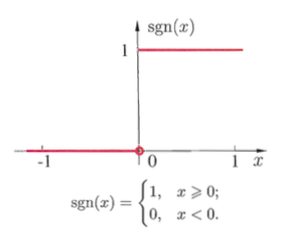
\includegraphics[width=2in]{figures/Heaviside.png}   
      	\caption{Heaviside activation function }
      \end{figure}
      
      But its discontinuity at $t=0$
      makes it difficult to use in practice. Instead we consider the
      following linear-step function:
  \begin{equation}\label{linear-step}
  \sigma(t)=
    \begin{cases}
       0 \quad t<0, \\
      t\quad 0\le t\le 1, \\
     1 \quad t> 1. \\
    \end{cases}
  \end{equation}
\begin{figure}
\centering
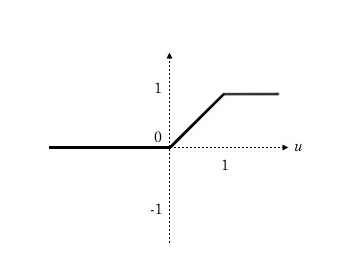
\includegraphics[width=2in]{./figures/zig}   
\caption{Linear-step function}
\end{figure}
This $\sigma(t)$ is closely related to the so-called Rectified Linear Unit function: 
\begin{equation}\label{ReLU}
ReLU(t):=\begin{cases}
0 \quad t< 0, \\
t \quad t\ge 0. 
\end{cases}
\end{equation}
\begin{figure}
\centering
\includegraphics[width=2in]{./figures/ReLU}   
\caption{ReLU activation function }
\end{figure}
Namely 
\begin{equation}
  \label{sigma-ReLU}
\sigma(t)=ReLU(t)-ReLU(t-1).
\end{equation}

\begin{lemma}
	If $A_1$, $A_2\subset\mathbb{R}^n$ are linearly separable, then there exist $w\in\mathbb{R}^{1\times n}$, $b\in\mathbb{R}$ such that
	\begin{equation}
	f(x):=\left( \begin{array}{cc}
	\sigma(wx+b) \\
	\sigma(-(wx+b))
	\end{array}
	\right)
	= e_i,\quad\mathrm{if}\ x\in A_i,\ i=1,2.
	\end{equation}
\end{lemma}
\begin{proof}
  By the definition of linearly separable sets, there exist
  $w_0\in\mathbb{R}^{1\times n}$, $b_0\in\mathbb{R}$ such that
  $w_0x+b_0>0$ if $x\in A_1$ and $w_0x+b_0<0$ if $x\in A_2$. We can
  find $\varepsilon>0$ such that
\begin{equation}
w_0x+b_0\begin{cases}
>\varepsilon \qquad x\in A_1, \\
<-\varepsilon \quad x\in A_2 .
\end{cases}
\end{equation}
Let $w=w_0/\varepsilon$, $b=b_0/\varepsilon$, we have:
\begin{equation}
wx+b\begin{cases}
>1 \qquad x\in A_1, \\
<-1 \quad x\in A_2 .
\end{cases}
\end{equation}
which implies $f(x)=e_i$ if $x\in A_i$.
\end{proof}

The extension of the above lemma to $k$-classes is straightforward.
\begin{lemma}
  If $A_i \subset \mathbb{R}^n(1\le i \le k)$ are linearly separable,
  there exist $W\in\mathbb{R}^{k\times n}$, $b\in\mathbb{R}^k$ s.t.
\begin{equation}
  \label{simple-f}
	f(x):=\sigma(Wx+b) = e_i,\quad\mathrm{for\ }x\in A_i  
\end{equation}
\end{lemma}

Oftentimes, we use the following notation
\begin{equation}
  \label{theta}
\theta=(W,b)\in\mathbb{R}^{k\times(n+1)} \mbox{ and } \theta[x]=Wx+b.
\end{equation}
